% =============================================================================
% STAR RPi5 Buildroot Implementation Primer
% Comprehensive Guide for Raspberry Pi 5 Custom Linux OS
% =============================================================================

\documentclass[11pt,letterpaper]{article}

\usepackage[utf8]{inputenc}
\usepackage[T1]{fontenc}
\usepackage{geometry}
\usepackage{graphicx}
\usepackage{hyperref}
\usepackage{listings}
\usepackage{xcolor}
\usepackage{fancyhdr}
\usepackage{titlesec}
\usepackage{booktabs}
\usepackage{longtable}
\usepackage{tabularx}
\usepackage{enumitem}
\usepackage{tikz}
\usepackage{float}

\usetikzlibrary{shapes.geometric, arrows.meta, positioning}

\geometry{margin=1in}

\hypersetup{
    colorlinks=true,
    linkcolor=blue!70!black,
    urlcolor=cyan!70!black,
    pdftitle={STAR RPi5 Buildroot Implementation Primer},
}

\definecolor{codebg}{RGB}{245,245,245}
\definecolor{codeframe}{RGB}{200,200,200}
\definecolor{codekey}{RGB}{0,0,180}
\definecolor{codecomment}{RGB}{0,128,0}
\definecolor{codestring}{RGB}{163,21,21}

\lstset{
    basicstyle=\ttfamily\small,
    backgroundcolor=\color{codebg},
    frame=single,
    rulecolor=\color{codeframe},
    breaklines=true,
    tabsize=2,
    showstringspaces=false,
    numbers=left,
    numberstyle=\tiny\color{gray},
    keywordstyle=\color{codekey}\bfseries,
    commentstyle=\color{codecomment}\itshape,
    stringstyle=\color{codestring},
}

\lstdefinelanguage{yaml}{
    keywords={true, false, null, yes, no},
    morecomment=[l]{\#},
    morestring=[b]',
    morestring=[b]",
    sensitive=true,
}

\lstdefinelanguage{ini}{
    morecomment=[s][\color{gray}]{[}{]},
    morecomment=[l]{\#},
    morecomment=[l]{;},
}

\pagestyle{fancy}
\fancyhf{}
\fancyhead[L]{\leftmark}
\fancyhead[R]{STAR RPi5 Buildroot Primer}
\fancyfoot[C]{\thepage}

\title{\textbf{STAR RPi5 Buildroot Implementation Primer}\\[0.5cm]
\large Custom Linux OS for Raspberry Pi 5 Robot Platform}
\author{STAR Development Team}
\date{December 2025}

\begin{document}

\maketitle
\tableofcontents
\newpage

% =============================================================================
\section{Project Overview}
% =============================================================================

\subsection{Purpose}

The \texttt{star-rpi5-buildroot} project creates a custom, minimal Linux distribution for the Raspberry Pi 5. It includes ROS 2, SLAM algorithms, navigation stack, and all dependencies needed for the STAR robot.

\subsection{Current Implementation Status}

\begin{table}[H]
\centering
\begin{tabular}{|l|c|l|}
\hline
\textbf{Component} & \textbf{Status} & \textbf{Notes} \\
\hline
Buildroot Base & Complete & 2025.02 LTS, ARM64 \\
Kernel Config & Complete & Linux 6.6 for Pi5 \\
WiFi Dual-Mode & Complete & Station + Access Point \\
mDNS Discovery & Complete & star-robot.local via Avahi \\
OpenCV + Python & Complete & ML stack ready \\
Camera Support & Complete & libcamera, V4L2 \\
systemd Services & Complete & Network, gateway templates \\
\hline
ROS 2 Jazzy & \textbf{Placeholder} & Directory structure only \\
SLAM Toolbox & \textbf{TODO} & Package not integrated \\
Nav2 Stack & \textbf{TODO} & Navigation packages needed \\
star-gateway & \textbf{TODO} & Spring Boot application \\
LiDAR Drivers & \textbf{TODO} & rplidar\_ros2, sick\_scan\_xd \\
\hline
\end{tabular}
\caption{Implementation Status Summary}
\end{table}

\subsection{Network Architecture}

\begin{figure}[H]
\centering
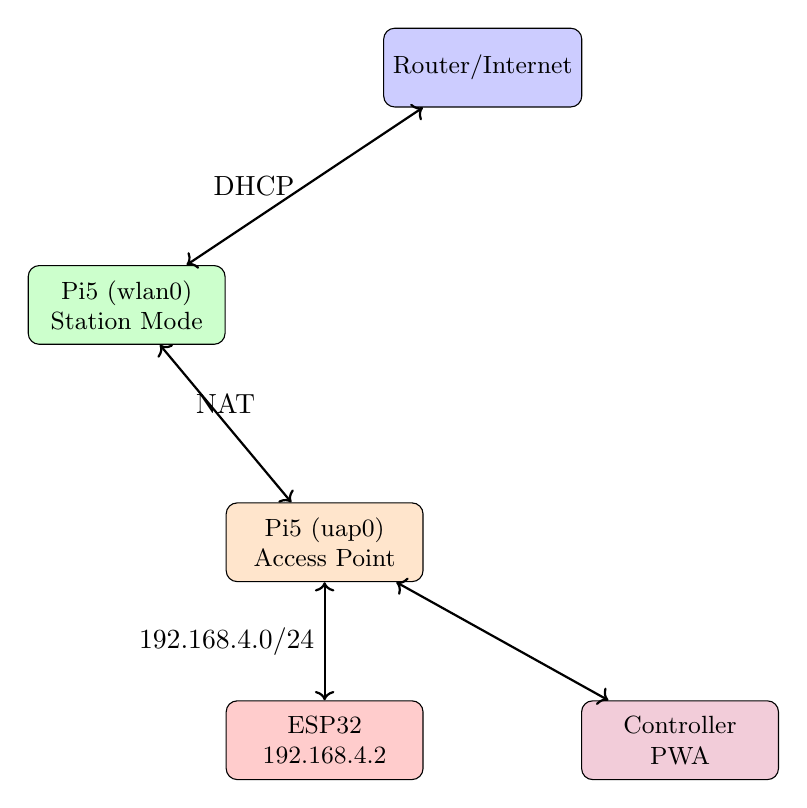
\begin{tikzpicture}[
    node distance=1.5cm,
    box/.style={draw, rectangle, rounded corners, minimum width=2.5cm, minimum height=1cm, align=center, font=\small},
    arrow/.style={->, thick}
]
    \node[box, fill=blue!20] (internet) {Router/Internet};
    \node[box, fill=green!20, below left=2cm and 2cm of internet] (pi5sta) {Pi5 (wlan0)\\Station Mode};
    \node[box, fill=orange!20, below right=2cm and 0cm of pi5sta] (pi5ap) {Pi5 (uap0)\\Access Point};
    \node[box, fill=red!20, below=1.5cm of pi5ap] (esp32) {ESP32\\192.168.4.2};
    \node[box, fill=purple!20, right=2cm of esp32] (controller) {Controller\\PWA};

    \draw[arrow, <->] (internet) -- node[left] {DHCP} (pi5sta);
    \draw[arrow, <->] (pi5sta) -- node[above] {NAT} (pi5ap);
    \draw[arrow, <->] (pi5ap) -- node[left] {192.168.4.0/24} (esp32);
    \draw[arrow, <->] (pi5ap) -- (controller);
\end{tikzpicture}
\caption{Dual WiFi Network Topology}
\end{figure}

% =============================================================================
\section{Directory Structure}
% =============================================================================

\begin{lstlisting}[language=bash]
star-rpi5-buildroot/
|-- Makefile                      # Build orchestration
|-- README.md                     # User documentation
|-- Config.in                     # External tree config
|-- external.desc                 # Buildroot external desc
|-- external.mk                   # Package includes
|
|-- configs/
|   |-- rpi5_64_defconfig         # Main Buildroot config
|   |-- config.txt                # Pi5 boot config
|   +-- busybox.config            # Minimal busybox
|
|-- package/
|   +-- ros2-jazzy/               # ROS 2 package (placeholder)
|       |-- Config.in
|       +-- ros2-jazzy.mk
|
|-- overlays/                     # Rootfs customizations
|   |-- etc/
|   |   |-- hostapd/              # WiFi AP config
|   |   |-- wpa_supplicant/       # WiFi station config
|   |   |-- dnsmasq.d/            # DHCP for AP
|   |   |-- iptables/             # NAT rules
|   |   |-- systemd/system/       # Service files
|   |   +-- profile.d/            # Environment scripts
|   +-- root/
|       +-- setup-network.sh      # Interactive setup
|
+-- scripts/
    |-- post-build.sh             # Enable services
    |-- post-image.sh             # Generate SD image
    +-- qemu-test.sh              # QEMU testing
\end{lstlisting}

% =============================================================================
\section{Implementation Tasks}
% =============================================================================

\subsection{Phase 1: ROS 2 Integration}

\subsubsection{Task 1.1: ROS 2 Jazzy Binary Integration}

The current \texttt{ros2-jazzy} package is a placeholder. Implement actual binary installation:

\textbf{Option A: Pre-built ARM64 Binaries}

\begin{enumerate}
    \item Download ROS 2 Jazzy ARM64 binaries from OSRF
    \item Create Buildroot package that extracts to \texttt{/opt/ros/jazzy}
    \item Handle dependencies (Python packages, shared libraries)
    \item Test with \texttt{ros2 run demo\_nodes\_cpp talker}
\end{enumerate}

\begin{lstlisting}[language=make, caption=ros2-jazzy.mk (Binary Installation)]
ROS2_JAZZY_VERSION = jazzy
ROS2_JAZZY_SOURCE = ros2-jazzy-$(ROS2_JAZZY_VERSION)-linux-arm64.tar.bz2
ROS2_JAZZY_SITE = https://github.com/ros2/ros2/releases/download/...

define ROS2_JAZZY_INSTALL_TARGET_CMDS
    mkdir -p $(TARGET_DIR)/opt/ros/jazzy
    tar -xf $(@D)/$(ROS2_JAZZY_SOURCE) -C $(TARGET_DIR)/opt/ros/jazzy
endef

$(eval $(generic-package))
\end{lstlisting}

\textbf{Option B: Build from Source (More Complex)}

\begin{enumerate}
    \item Add colcon build system to Buildroot
    \item Cross-compile ROS 2 base packages
    \item Handle CMake cross-compilation settings
    \item Much longer build time (2+ hours)
\end{enumerate}

\subsubsection{Task 1.2: SLAM Toolbox Package}

Create \texttt{package/slam-toolbox/}:

\begin{lstlisting}[language=make, caption=slam-toolbox.mk]
SLAM_TOOLBOX_VERSION = jazzy
SLAM_TOOLBOX_SITE = $(call github,SteveMacenski,slam_toolbox,$(SLAM_TOOLBOX_VERSION))
SLAM_TOOLBOX_DEPENDENCIES = ros2-jazzy eigen boost

define SLAM_TOOLBOX_BUILD_CMDS
    source /opt/ros/jazzy/setup.bash && \
    cd $(@D) && colcon build --packages-select slam_toolbox
endef

$(eval $(generic-package))
\end{lstlisting}

\subsubsection{Task 1.3: Nav2 Navigation Stack}

Create \texttt{package/nav2/}:

Required packages:
\begin{itemize}
    \item nav2\_bringup
    \item nav2\_bt\_navigator
    \item nav2\_planner
    \item nav2\_controller
    \item nav2\_costmap\_2d
    \item nav2\_amcl
    \item dwb\_core (DWA local planner)
\end{itemize}

\subsection{Phase 2: LiDAR Integration}

\subsubsection{Task 2.1: RPLiDAR Driver}

Create \texttt{package/rplidar-ros2/}:

\begin{enumerate}
    \item Clone rplidar\_ros2 from Slamtec
    \item Build as ROS 2 package
    \item Configure for UART: \texttt{/dev/ttyUSB0} at 460800 baud
    \item Test with \texttt{ros2 launch rplidar\_ros2 rplidar\_c1\_launch.py}
\end{enumerate}

\subsubsection{Task 2.2: SICK TiM561 Driver}

Create \texttt{package/sick-scan-xd/}:

\begin{enumerate}
    \item Clone sick\_scan\_xd from SICK AG
    \item Build as ROS 2 package
    \item Configure for Ethernet: \texttt{192.168.0.1:2112}
    \item Test with \texttt{ros2 launch sick\_scan\_xd sick\_tim\_5xx.launch.py}
\end{enumerate}

\subsection{Phase 3: star-gateway Integration}

\subsubsection{Task 3.1: Java Runtime}

Add OpenJDK 17 to Buildroot:

\begin{lstlisting}[language=bash, caption=Add to rpi5\_64\_defconfig]
BR2_PACKAGE_OPENJDK=y
BR2_PACKAGE_OPENJDK_VERSION_17=y
\end{lstlisting}

Note: OpenJDK build may fail on WSL. Use native Linux or pre-built binaries.

\subsubsection{Task 3.2: Gateway Deployment}

Update \texttt{overlays/etc/systemd/system/robot-gateway.service}:

\begin{lstlisting}[language=ini, caption=robot-gateway.service]
[Unit]
Description=STAR Robot Gateway
After=network-online.target ros2.service
Wants=network-online.target

[Service]
Type=simple
User=root
WorkingDirectory=/opt/star-gateway
ExecStart=/usr/bin/java -Xmx512m -jar star-gateway.jar
Environment="JAVA_HOME=/usr/lib/jvm/java-17-openjdk"
Environment="ROS_DISTRO=jazzy"
Environment="ROS_DOMAIN_ID=0"
Restart=always
RestartSec=10

[Install]
WantedBy=multi-user.target
\end{lstlisting}

\subsubsection{Task 3.3: Gateway Build Script}

Create deployment pipeline:

\begin{lstlisting}[language=bash, caption=deploy-gateway.sh]
#!/bin/bash
# Build and deploy star-gateway to Pi5

# Build JAR
cd ../star-gateway
./gradlew bootJar

# Copy to Pi5
scp build/libs/star-gateway-*.jar root@star-robot.local:/opt/star-gateway/star-gateway.jar

# Restart service
ssh root@star-robot.local "systemctl restart robot-gateway"
\end{lstlisting}

\subsection{Phase 4: System Configuration}

\subsubsection{Task 4.1: ROS 2 Launch Files}

Create \texttt{overlays/opt/ros/star\_bringup/}:

\begin{lstlisting}[language=python, caption=star\_robot.launch.py]
from launch import LaunchDescription
from launch_ros.actions import Node

def generate_launch_description():
    return LaunchDescription([
        # LiDAR driver
        Node(
            package='rplidar_ros2',
            executable='rplidar_node',
            parameters=[{'serial_port': '/dev/ttyUSB0',
                        'frame_id': 'laser_frame'}]
        ),
        # SLAM Toolbox
        Node(
            package='slam_toolbox',
            executable='async_slam_toolbox_node',
            parameters=['slam_params.yaml']
        ),
        # Nav2 stack
        IncludeLaunchDescription(
            PythonLaunchDescriptionSource('nav2_bringup/launch/navigation_launch.py'),
            launch_arguments={'params_file': 'nav2_params.yaml'}.items()
        ),
    ])
\end{lstlisting}

\subsubsection{Task 4.2: SLAM Parameters}

Create \texttt{overlays/opt/ros/config/slam\_params.yaml}:

\begin{lstlisting}[language=yaml, caption=slam\_params.yaml]
slam_toolbox:
  ros__parameters:
    solver_plugin: solver_plugins::CeresSolver
    ceres_linear_solver: SPARSE_NORMAL_CHOLESKY

    odom_frame: odom
    map_frame: map
    base_frame: base_link
    scan_topic: /scan

    resolution: 0.05              # 5cm per cell
    max_laser_range: 12.0         # RPLiDAR C1 max
    minimum_travel_distance: 0.3
    minimum_travel_heading: 0.3

    do_loop_closing: true
    loop_search_maximum_distance: 3.0

    # Performance tuning for RPi5
    transform_publish_period: 0.05  # 20 Hz
    map_update_interval: 0.5        # 2 Hz
\end{lstlisting}

\subsubsection{Task 4.3: Nav2 Parameters}

Create \texttt{overlays/opt/ros/config/nav2\_params.yaml}:

\begin{lstlisting}[language=yaml, caption=nav2\_params.yaml (DWA Controller)]
controller_server:
  ros__parameters:
    controller_frequency: 20.0
    FollowPath:
      plugin: "dwb_core::DWBLocalPlanner"
      max_vel_x: 0.5
      min_vel_x: -0.3
      max_vel_theta: 1.0
      acc_lim_x: 1.0
      acc_lim_theta: 2.0
      decel_lim_x: -1.5
      vx_samples: 20
      vtheta_samples: 40
      sim_time: 1.5
      critics: ["RotateToGoal", "Oscillation", "BaseObstacle",
                "GoalAlign", "PathAlign", "PathDist", "GoalDist"]
\end{lstlisting}

% =============================================================================
\section{Build Instructions}
% =============================================================================

\subsection{Prerequisites}

\begin{lstlisting}[language=bash]
# Ubuntu/Debian dependencies
sudo apt-get install build-essential libncurses5-dev git \
    bc bison flex libssl-dev make unzip wget cpio rsync

# Disk space: ~20GB free
# Build time: 1-2 hours (first build)
\end{lstlisting}

\subsection{Build Commands}

\begin{lstlisting}[language=bash]
cd star-rpi5-buildroot

# Full build (download + configure + build)
make build

# Or step-by-step:
make download      # Get Buildroot 2025.02
make configure     # Apply our config
make              # Build everything

# Output: buildroot-2025.02/output/images/sdcard.img
\end{lstlisting}

\subsection{Flash to SD Card}

\begin{lstlisting}[language=bash]
# Find SD card device (e.g., /dev/sdb)
lsblk

# Flash image (CAUTION: double-check device!)
sudo dd if=buildroot-2025.02/output/images/sdcard.img \
    of=/dev/sdX bs=4M status=progress
sync
\end{lstlisting}

\subsection{First Boot Setup}

\begin{lstlisting}[language=bash]
# Connect via Ethernet or serial console
ssh root@<IP_ADDRESS>  # No password

# Or via mDNS (after network configured)
ssh root@star-robot.local

# Run interactive network setup
/root/setup-network.sh
# Choose option 8 for full setup
\end{lstlisting}

% =============================================================================
\section{Testing}
% =============================================================================

\subsection{QEMU Testing}

Test without hardware using QEMU:

\begin{lstlisting}[language=bash]
# Serial console boot
make qemu

# Graphical mode (VNC)
make qemu-graphical

# SSH into QEMU instance
make qemu-ssh
\end{lstlisting}

Note: QEMU uses generic ARM64 machine, not Pi5-specific. Good for testing systemd, networking, userspace.

\subsection{Hardware Testing Checklist}

\begin{enumerate}
    \item Boot Pi5, verify serial console output
    \item Check WiFi station connects to router
    \item Check WiFi AP creates STAR-Robot-AP network
    \item Verify ESP32 can connect to AP
    \item Test mDNS: \texttt{ping star-robot.local}
    \item Test SSH access
    \item Verify camera: \texttt{libcamera-hello}
    \item Test ROS 2: \texttt{ros2 topic list}
    \item Run SLAM with LiDAR
    \item Test star-gateway API endpoints
\end{enumerate}

% =============================================================================
\section{Troubleshooting}
% =============================================================================

\subsection{Common Issues}

\begin{description}
    \item[Build fails on WSL] OpenJDK cross-compilation doesn't work. Use native Linux or remove Java from config.

    \item[WiFi AP not starting] Check \texttt{systemctl status hostapd}. May need to manually create uap0 interface.

    \item[ROS 2 not found] The ros2-jazzy package is a placeholder. Install ROS 2 manually after first boot.

    \item[SSH permission denied] Default config allows empty root password. If changed, use the password you set.
\end{description}

\subsection{Debugging Commands}

\begin{lstlisting}[language=bash]
# Check service status
systemctl status hostapd dnsmasq-ap wifi-nat wpa_supplicant@wlan0

# View logs
journalctl -u robot-gateway -f

# Network interfaces
ip addr show
iwconfig

# ROS 2 environment
source /opt/ros/jazzy/setup.bash
ros2 doctor
\end{lstlisting}

% =============================================================================
\section{References}
% =============================================================================

\begin{itemize}
    \item Buildroot Manual: \url{https://buildroot.org/downloads/manual/manual.html}
    \item ROS 2 Jazzy Installation: \url{https://docs.ros.org/en/jazzy/Installation.html}
    \item SLAM Toolbox: \url{https://github.com/SteveMacenski/slam_toolbox}
    \item Nav2 Documentation: \url{https://docs.nav2.org/}
    \item RPLiDAR ROS 2: \url{https://github.com/Slamtec/rplidar_ros}
    \item STAR FTP Section 17: Software Implementation
    \item STAR Software Architecture Primer: Sections 5, 14
\end{itemize}

\end{document}
